\documentclass{article}

\usepackage{arxiv}
% RETTET: Tilføjet ] og ændret til numeric, så du kan lave hævede tal
\usepackage[backend=biber, style=numeric]{biblatex} 
\addbibresource{kilder.bib} 

\usepackage[utf8]{inputenc} 
\usepackage[T1]{fontenc} % RETTET: De usynlige mellemrum er renset væk
\usepackage{hyperref}       % hyperlinks
\usepackage{url}            % simple URL typesetting
\usepackage{booktabs}       % professional-quality tables
\usepackage{amsfonts}       % blackboard math symbols
\usepackage{nicefrac}       % compact symbols for 1/2, etc.
\usepackage{microtype}      % microtypography
\usepackage{graphicx}
\usepackage{float}
\usepackage{doi}
\usepackage{amsmath}

\title{Multimodal capabilities of Gemma-4-E2B}

\author{
    Rune Christensen\\
    Artificial Intelligence \& Data  \\
    DTU \\
    \texttt{s250910@dtu.dk} \\
    \And
    Anas Alkaisi\\
    Artificial Intelligence and Data\\
    DTU \\
    \texttt{s255797@dtu.dk} \\
    \And
    Frederik Naervig Gerlach-Hansen \\
    Artificial Intelligence \& Data \\
    DTU \\
    \texttt{s256931@dtu.dk} \\
}

% Uncomment to remove the date
%\date{}

\renewcommand{\shorttitle}{Multimodal capabilities of Gemma-4-E2B}

%%% Add PDF metadata
\hypersetup{
pdftitle={Multimodel capabilities of open source models},
pdfsubject={},
pdfauthor={},
pdfkeywords={},
}

\begin{document}
\maketitle

\begin{abstract}
Large language models are becoming increasingly common tools among students, but how well do they actually perform on real university-level exams? This project investigates exactly that, by testing Gemma, an open-source, locally run language model on multiple-choice questions from DTU's course 02450 ''Introduction to Machine Learning and Data Mining''.
Our main question is whether Gemma performs better on questions presented in different formats. We split exam questions into three categories: pure text questions, questions containing figures or plots (given as screenshots), and questions containing tables or matrices with numerical data (given both as screenshots and as written descriptions). This last category lets us directly compare whether Gemma does better when it reads the numbers from a table versus seeing it visually, while for figures and plots, a screenshot is the only reasonable way to present the information.
We sourced our data from past 02450 exam sets and used a consistent prompt across all questions, framing Gemma as a student sitting a university exam. Responses were scored against official answer keys, with accuracy as our main metric.
Beyond just measuring how well Gemma scores, we're also interested in what kinds of mistakes it makes — and whether those patterns reveal something about the limits of open-source, locally deployed models for academic use.
\end{abstract}



\newpage

\section{Introduction}
The rapid advancement of generative artificial intelligence has raised important questions regarding its impact on education and assessment. Modern AI systems are increasingly capable of solving complex academic tasks, including multiple-choice examination questions, which has led to concerns about academic integrity and the potential misuse of AI during unsupervised assessments. This can be seen in the "Generative AI use and misuse call for assessment reform in higher education"\supercite{chirikov2026genai} article published in Science. According to this article 9\% of undergrad students admit to using AI to cheat. At the same time, locally deployable models have become widely accessible, making it possible for students to run powerful AI systems directly on their personal computers without relying on cloud-based services. Understanding the capabilities and limitations of such models is therefore becoming increasingly relevant for both educators and students.

Motivated by these developments, this report investigates the performance of the locally deployable AI model Gemma-4-e2b on multiple-choice examination sets from the DTU course Introduction to Machine Learning and Data Mining (02450, 02452). Specifically, the study tests whether the model answers fewer questions correctly when a figure or table is shown as an image than when the same information is given as text. This addresses the multimodal evaluation gap described in Section~3.3 (p.~14) of "Sociotechnical Safety Evaluation of Generative AI Systems"\supercite{weidinger2023sociotechnical}. This is done to show the strengths and weaknesses of a locally run open-source model like Gemma, and to find out which kinds of questions are more AI-resistant: those given as text, or those that rely on figures and tables.

To evaluate the model, Gemma was tested on 16 publicly available examination sets spanning the years 2017–2025. Each exam set contains 27 multiple-choice questions, giving 432 distinct questions in total. A central objective of the study was to compare Gemma's performance on image-based and text-based prompts. For questions containing graphical visualizations, the model was evaluated under two separate conditions. In the first condition, Gemma received a screenshot of the visualization together with the original question text. In the second condition, the visualization was replaced by a detailed textual description generated using Anthropics Fable 5 model, while the original question text remained unchanged. This experimental setup allowed for a direct comparison of the model's ability to interpret graphical information versus equivalent textual descriptions.

The findings of this study provide insight into the practical capabilities of a locally run model like Gemma in an academic setting and contribute to the broader discussion surrounding the role of generative AI in modern education.



\section{Methods}
\subsection{The Dataset}

The dataset employed in this study consists of publicly available examination sets from the DTU course \textit{Introduction to Machine Learning and Data Mining} (02450 and 02452) spanning the years 2017-2025. Both the spring and fall examinations were included, resulting in a total of 16 exam sets. Each examination contains 27 multiple-choice questions, yielding a total sample size of 432 questions. These are real exams used to assess students, and each set is published together with an official solution, which we used as the answer key. Every question has exactly one correct answer, and the exams cover the course curriculum, including data preprocessing, clustering, classification, regression, and model evaluation.

The 432 questions differ in how the information needed to answer them is presented. 141 can be answered from text alone, 157 rely on a figure or plot --- such as a scatter plot, dendrogram, or ROC curve --- that cannot be faithfully written out as text, and the remaining 134 contain a table or matrix of numbers that can be presented either as an image or written out as text. The image versions of all figures and tables were cropped directly from the original exam PDFs.


\subsection{The Experimental Setup}

The objective of the experiment was to evaluate Gemma's ability to answer multiple-choice examination questions presented through different information modalities. The four different input modalities are presented below.

\begin{itemize}
    \item \textbf{Unpaired questions}: the question is presented in a single modality.
    \begin{itemize}
        \item \textbf{Unpaired text}: all the information needed is text. Gemma received the question text and answer options.
        \item \textbf{Unpaired image}: the information is presented only through a visual element such as a graph, figure, or diagram that cannot be written out as text. Gemma received it as a screenshot together with the question text and answer options.
    \end{itemize}
    \item \textbf{Paired questions}: the question contains information that can be given both as text and as a screenshot, e.g. a matrix, vector, or table.
    \begin{itemize}
        \item \textbf{Paired text}: the visual element was first converted into a detailed textual description using Claude's Fable 5. Gemma received this description together with the original question text and answer options.
        \item \textbf{Paired image}: Gemma received the original question text, answer options, and a screenshot of the associated visual element.
    \end{itemize}
\end{itemize}

\small{See appendix for examples of each question category}\newline


Unpaired examination questions can be considered independent, as each question is evaluated separately and does not share observations with other questions. Consequently, they produce unpaired (independent) observations. In contrast, the paired question is evaluated under both prompt modalities, resulting in paired observations. This pairing allows for a direct comparison between modalities using McNemar’s test as further explained in section 2.4.2.

The outcome metric in all analyses is accuracy, the proportion of questions answered correctly. Because each question has exactly one correct answer, the outcome is binary (correct or incorrect), and the dataset is not imbalanced, accuracy provides an appropriate measure of performance. This matters because accuracy can be misleading for imbalanced data, where precision and recall are preferred instead, as shown in slide~5 of the Day~4 lecture material\supercite{das2026day4}.


\subsubsection{Prompting Strategy}

To obtain consistent and comparable responses across all questions, the same prompt structure was used throughout the experiment. Each question was submitted to Gemma with an instruction to reason through the problem step by step before providing a final answer. Without this explicit instruction, Gemma wouldn't use chain of thought and it would produce notably worse results. The model was required to end every response with the line \texttt{FINAL ANSWER: X}, where X is one of the answer options A--E. This format allowed the final answer to be extracted automatically from the model output.

To ensure reproducibility, Gemma was run using greedy decoding, meaning that the most likely next token was always selected rather than sampling from a probability distribution. Consequently, repeated evaluations of the same prompt produced identical outputs.

The option E was included in every question as a ``don't know'' option, allowing Gemma to express uncertainty rather than being forced to guess. Since E was never the correct answer for any question, random guessing among the four valid options A--D yields a baseline accuracy of 25\%, which serves as the reference value in the binomial tests.

The prompt provided to Gemma was:

\begin{quote}
``You are answering a multiple-choice exam question from a university Machine Learning course. Each question has exactly one correct answer among A, B, C, D. You may also answer E if you genuinely do not know. Think the problem through step by step: write out your reasoning and any calculations first, but keep each step short and to the point. ALWAYS finish your reply with one line of exactly this form: FINAL ANSWER: X where X is a single capital letter A, B, C, D, or E.''
\end{quote}

Depending on the experimental condition described in Section 2.2, either textual content or visual information was appended to this prompt before being submitted to Gemma.

\subsection{The Model}
The model used in the project is Gemma-4-E2B. It is an open source language model developed by Google DeepMind. Gemma 4 is a multimodal model capable of processing both textual and visual inputs, making it suitable for the experimental design of this study, which involves both text and image processing. The model was selected due to its strong performance among open-source large language models. In official documentation, Google describes the Gemma family as “frontier-level performance at each size.”\supercite{gemma4modelcard}

Unlike closed models such as ChatGPT or Claude, Gemma 4 is released under an Apache 2.0 license, meaning it can be downloaded, run locally, and used freely. This was important for the project, since it allowed all experiments to be run on a local machine with full control over the setup, without any API calls and with no concerns about data leaving the local environment.

Running the model locally also made it straightforward to ensure statistical independence between observations, as each question could be sent in a completely fresh session with no shared state between calls. This follows the design used to ensure independence in Appendix~C.1 (p.~17) of "Evaluation of Large Language Models: STEM Education and Gender Stereotypes"\supercite{due2024evaluation}.\newline

The Gemma family consists of models of varying size, ranging from 2 to 31 billion parameters. The 2 billion parameter model (Gemma-4-E2B) was chosen so that the study could be reproduced by anyone with a normal computer. It was run on a desktop PC with 16 GB of VRAM. Of that 16 GB it used roughly 10 GB. A typical student laptop, for example a MacBook Air with 16 GB of unified memory, could therefore run it pretty comfortably.
\newline

Gemma 4 has a knowledge cutoff of January 2025\supercite{gemma4modelcard}, which introduces a potential problem. Any exam set published before this date may have been part of the model's training data, in which case Gemma would not be solving these questions itself, but it would rely on information it has already seen. This problem is known as data contamination, which is discussed as a limitation of benchmarks in Section~8.3 (p.~56) of "Evaluating Large Language Models: A Comprehensive Survey"\supercite{guo2023evaluating}, and would be a huge problem for this study, as it would inflate the accuracy scores of the exams before January 2025. This inflation of accuracy only affects exam sets from before the cutoff, but it doesn't affect exam sets after the cutoff.
To account for this, we subsequently perform a one-sided two-proportion z-test comparing the success rates on exam sets from before and after January 2025. This test provides evidence as to whether there is a statistically significant difference in performance between the two periods, which may indicate whether the pre-2025 exam material was included in Gemma’s training data.



\subsection{Statistical methods}

\subsubsection{Confidence intervals}

All accuracy estimates are reported with a 95\% confidence interval. Since each accuracy is a proportion of correct answers, we use the normal-approximation interval

$$\hat{p} \pm 1.96\sqrt{\frac{\hat{p}(1-\hat{p})}{n}},$$

where $\hat{p}$ is the observed accuracy and $n$ is the number of questions. The value $1.96$ is the $97.5\%$ quantile of the standard normal distribution. The test is valid if $np > 15$ and $n(1-p) > 15$; that is, the expected numbers of successes and failures must each be greater than $15$.

\subsubsection{McNemar's test}

McNemar's test was used to compare performance between the screenshot and text-description modalities for paired questions. Since the same questions were evaluated under both conditions, the resulting observations are paired, making McNemar's test an appropriate choice. Furthermore, the model output is binary (success/failure), corresponding to nominal data, which satisfies one of the assumptions of the test. McNemar's test is also a non-parametric procedure, meaning that it does not rely on distributional assumptions regarding the underlying population. We employed the chi-squared approximation version of the test, as described in Section 4.3 of "Model Evaluation, Model Selection, and Algorithm Selection in Machine Learning"\supercite{raschka2018model}

The McNemar test is used to compare two paired methods when the outcome for each observation is binary (e.g., success or failure). Since both methods are applied to the same set of observations, the results are not independent and therefore cannot be analyzed using a standard two-sample proportion test. 

The paired outcomes are summarized in a $2\times2$ contingency table:

\begin{center}
\begin{tabular}{c c c c}
&
&
\multicolumn{2}{c}{\textbf{Method A}} \\
\cline{3-4}
&
&
\textbf{Success}
&
\textbf{Failure}
\\
\cline{2-4}
\multirow{}{}{\rotatebox[origin=c]{90}{\textbf{Method B}}}
&
\textbf{Success}
&
$a$
&
$b$
\\
&
\textbf{Failure}
&
$c$
&
$d$
\\
\cline{2-4}
\end{tabular}
\end{center}

The diagonal cells ($a$) and ($d$) contain the concordant pairs, where both methods produce the same outcome. These observations provide no evidence of a difference between the methods. Instead, McNemar's test focuses exclusively on the discordant pairs ($b$) and ($c$), which correspond to observations for which the two methods disagree. Under the null hypothesis,
$$
H_0 : p = 0.5,
$$

each method is equally likely to be correct among the discordant pairs. Consequently, conditional on the total number of discordant pairs ($n=b+c$), the number of observations in cell ($b$) follows a binomial distribution,

$$
b \sim \mathrm{Binomial}(n=b+c, p=0.5).
$$

For sufficiently large values when ($b+c \ge 25$), the McNemar test statistic

$$
\chi^2=\frac{(b-c)^2}{b+c}
$$

approximately follows a chi-squared distribution with one degree of freedom under ($H_0$). For smaller samples, a continuity-corrected version known as Edwards' correction,

$$
\chi^2=\frac{(|b-c|-1)^2}{b+c},
$$

or the exact McNemar test based on the binomial distribution may be preferred.

Since this report utilizes the chi-squared approximation method the corresponding $p$-value is found as:

$$p_{value} = P(\chi^2 > \chi^2_{obs})$$

A small $p$-value indicates that the observed imbalance between ($b$) and ($c$) is unlikely to have occurred by chance, providing evidence that one method tends to outperform the other on the paired observations.

\subsubsection{Binomial tests}

This study performs 12 binomial tests in total. 6 of them assess whether Gemma's accuracy exceeded the 25\% baseline expected under random guessing in a four-option multiple-choice setting. The last two of these being full-exam simulations with multiple modalities combined. The other 6 binomial tests assess whether Gemma could pass the exam, i.e. whether its accuracy exceeded the 50\% threshold. The last two of these were also full-exam simulations. \newline 
For the two full-exam simulations; The first combines the unpaired text, unpaired image and paired-text questions, the second combines the unpaired text, unpaired image and paired-image questions\newline
All of these were one-sided tests since the purpose was to see how much better Gemma was than the guessing baseline/passing threshold.

The assumptions of a binomial test are 1) The outcomes should be binary, correct/incorrect, 2) Independent trials, the outcome of one trial shouldn't have an effect on the next one, 3) The probability for correct shouldn't change between trials. All of these assumptions are met in this study, and therefore a binomial test is a suitable test to check if the answers from Gemma are better than random guessing.\newline
\newline
The null hypothesis $H_0$ for a one-sided binomial test is $p_0=p$, and the alternative hypothesis $H_1$ is $p_0<p$\newline
The next step is to calculate the $p$-value. The CDF of a binomial distribution gives the probability of getting at most $x$ successes out of $n$ draws:

$$F(x) = P(X \le x) = \sum_{k=0}^{\lfloor x \rfloor} \binom{n}{k} p_0^{k} (1 - p_0)^{n-k}$$

Because the test is one-sided, we need the probability of getting at least as many correct answers as observed, which is the upper tail. The one-tailed p-value is therefore computed as:

$$p_{value} = P(X \ge x) = 1 - F(x-1)$$

Since each family contains six binomial tests asking the same question, there is a risk that one of them returns
a significant result purely by chance. Running $m$ tests each at $\alpha = 0.05$ 
raises the family-wise false positive rate to approximately $1 - 0.95^m$, so we 
apply the Bonferroni correction to control for this. The correction simply 
divides the significance threshold by the number of tests in the family:

\[
    \alpha_{\text{Bonf}} = \frac{\alpha}{m} = \frac{0.05}{6} = 0.00833
\]

This is the significance level we will compare our p-values to in the results section. Noteworthy, the Bonferroni method greatly reduces false positives (Type I errors) but increases the risk of missing true effects (Type II errors).

\subsubsection{Two-proportion z-test}

The two-proportion z-test is used in two places in this study. The first compares Gemma's accuracy on the unpaired text questions (given as text) with the unpaired image questions (given as screenshots), to see whether the format changes how well it does. This is a two-sided test. The second is a contamination check, which compares Gemma's accuracy on questions from before and after the model's knowledge cutoff, to see whether performance differs between the two time periods. This is done as a one-sided test.

The assumptions of a two-proportion z-test are 1) The outcomes should be binary, correct/incorrect, 2) The two groups should be independent, the questions in one group have no effect on the questions in the other, 3) The samples should be large enough for the normal approximation to hold, a common rule of thumb is the number of successes and failures must both be at least 10 respectively in each group. All of these assumptions are met in this study, and therefore a two-proportion z-test is a suitable test.\newline
\newline
The null hypothesis $H_0$ for the two-sided test is that the two groups have the same true accuracy, $p_1 = p_2$, and the alternative hypothesis $H_1$ is that the accuracies are different, $p_1 \neq p_2$. For the one-sided contamination check (before vs.\ after the knowledge cutoff) the hypotheses are instead directional, $H_0: p_{before} = p_{after}$ against $H_1: p_{before} > p_{after}$, testing specifically whether the pre-cutoff accuracy is inflated by training-data contamination.\newline
The test statistic is the difference between the two observed accuracies divided by the pooled standard error. Since the null hypothesis says the two accuracies are equal, the standard error is found from a pooled accuracy $\hat{p}$, which is the total number of correct answers in both groups divided by the total number of questions in both groups.

$$\hat{p} = \frac{x_1 + x_2}{n_1 + n_2}$$

where $x_1$ and $x_2$ are the number of correct answers and $n_1$ and $n_2$ the number of questions in each group. The pooled test statistic is then:

$$z_{obs} = \frac{\hat{p}_1 - \hat{p}_2}{\sqrt{\hat{p}(1 - \hat{p})\left(\frac{1}{n_1} + \frac{1}{n_2}\right)}}$$

Under $H_0$ the $z$-statistic follows a standard normal distribution, so the p-value can be found from it and compared to the significance level $\alpha = 0.05$.

\subsubsection{Power}

Since the dataset is fixed and numbers of questions can't be increased, the minimum effect-size detectable by the z-test at 80\% power and $\alpha = 0.05$ is now computed, following the sample-size formula for a difference in independent proportions given in slide~14 of the Day~4 lecture material\supercite{das2026day4}.

We start from the two-proportion sample-size formula, in which $p_1$ and $p_2$ are the true accuracies of the two groups,

$$n = \frac{(Z_{\alpha/2} + Z_{\beta})^2 \left[ p_1(1 - p_1) + p_2(1 - p_2) \right]}{(p_1 - p_2)^2}$$

and rearrange it to isolate the effect-size $p_1 - p_2$. Multiplying both sides by $(p_1 - p_2)^2$ and dividing by $n$,

$$(p_1 - p_2)^2 = \frac{(Z_{\alpha/2} + Z_{\beta})^2 \left[ p_1(1 - p_1) + p_2(1 - p_2) \right]}{n}$$

and taking the square root of both sides gives

$$p_1 - p_2 = (Z_{\alpha/2} + Z_{\beta})\sqrt{\frac{p_1(1 - p_1) + p_2(1 - p_2)}{n}}$$

To find the smallest effect-size detectable we set each term $p(1-p)$ at its maximum $0.25$, which occurs at $p = 0.5$. With $\alpha = 0.05$ (so $Z_{\alpha/2} = 1.96$), power $0.80$ (so $Z_{\beta} = 0.84$) and the smaller group size $n = 141$,

\begin{align*}
p_1 - p_2 &= (1.96 + 0.84)\sqrt{\frac{0.25 + 0.25}{141}} \\
&= 2.80 \cdot \sqrt{\frac{0.5}{141}} \\
&= 2.80 \cdot 0.0596 \\
&\approx 0.17
\end{align*}

So with this fixed $n$ the test can detect a true accuracy gap of $17$\% at least $80\%$ of the time. The gap that was observed in the Gemma run between the unpaired text and unpaired image questions is $0.738 - 0.376 = 0.36$, which is a lot higher than $0.17$. This means that the z-test is a good test to use in this study, and that it will almost always find a statistical significant difference between $p_{text}$ and $p_{graph}$ if there is one.

The same method was used for the contamination check. That test is one-sided (so $Z_{\alpha} = 1.645$) and its smaller group is the $n = 54$ post-cutoff 2025 questions, so
$$p_1 - p_2 = (1.645 + 0.84)\sqrt{\frac{0.25 + 0.25}{54}} \approx 0.24.$$
With only 54 post-cutoff questions the check is therefore only well-powered to detect a large pre-cutoff inflation (about $24$\% or more). The differences actually observed (about $17$\% when the paired questions are scored as images and $12$\% as text) are smaller than this and run the opposite way, so the non-significant result should be read with this limited power in mind.

\section{Results}

\subsection{Summary of the data}




\begin{table}[H]
\centering
\caption{Accuracy of the Gemma~4 run, with each question counted once. Each exam contains 27 distinct questions; the paired (figure/table) questions are shown either as an image or as a text description, so the full-exam totals and the by-date rows are reported under both presentations. The 134 paired questions are listed once under \emph{Paired text} and once under \emph{Paired image}, so the four input-format rows overlap and do not sum to the full-exam total ($432 = 141 + 157 + 134$). Accuracy is $n_{correct}/n_{total}$; 95\% confidence intervals use the normal approximation.}
\label{tab:accuracy-ci}
\begin{tabular}{lrrrr}
\toprule
\textbf{Group} & $n_{correct}$ & $n_{total}$ & \textbf{Accuracy} & \textbf{95\% CI} \\
\midrule
\multicolumn{5}{@{}l}{\textit{Accuracy by input format}} \\
Unpaired text   &  104 & 141 & 73.8\% & [66.5,\,81.0] \\
Unpaired image  &  59 & 157 & 37.6\% & [30.0,\,45.2] \\
Paired text     &  86 & 134 & 64.2\% & [56.1,\,72.3] \\
Paired image    &  60 & 134 & 44.8\% & [36.4,\,53.2] \\
\midrule
\multicolumn{5}{@{}l}{\textit{Full-exam accuracy --- each question counted once}} \\
Unpaired text + unpaired image + paired image & 223 & 432 & 51.6\% & [46.9,\,56.3] \\
Unpaired text + unpaired image + paired text  & 249 & 432 & 57.6\% & [53.0,\,62.3] \\
\midrule
\multicolumn{5}{@{}l}{\textit{Accuracy by exam date --- paired shown as image}} \\
Exams 2017--2024    & 187 & 378 & 49.5\% & [44.4,\,54.5] \\
Spring 2025         &  17 &  27 & 63.0\% & [44.7,\,81.2] \\
Fall 2025           &  19 &  27 & 70.4\% & [53.1,\,87.6] \\
2025 exams combined &  36 &  54 & 66.7\% & [54.1,\,79.2] \\
\midrule
\multicolumn{5}{@{}l}{\textit{Accuracy by exam date --- paired shown as text}} \\
Exams 2017--2024    & 212 & 378 & 56.1\% & [51.1,\,61.1] \\
Spring 2025         &  18 &  27 & 66.7\% & [48.9,\,84.4] \\
Fall 2025           &  19 &  27 & 70.4\% & [53.1,\,87.6] \\
2025 exams combined &  37 &  54 & 68.5\% & [56.1,\,80.9] \\
\bottomrule
\end{tabular}
\end{table}

\subsection{McNemar's test}

\begin{center}
\begin{tabular}{c c c c}
&
&
\multicolumn{2}{c}{\textbf{Paired text}} \\
\cline{3-4}
&
&
\textbf{Success}
&
\textbf{Failure}
\\
\cline{2-4}
\multirow{}{}{\rotatebox[origin=c]{90}{\textbf{Paired image}}}
&
\textbf{Success}
&
51
&
9
\\
&
\textbf{Failure}
&
35
&
39
\\
\cline{2-4}
\end{tabular}
\end{center}

\vspace{5ex}
The contingency table summarizes the paired outcomes for the 134 paired questions evaluated using both prompting methods. Both methods correctly answered 51 questions, while both methods incorrectly answered 39 questions.

The paired image method correctly answered 9 questions that the paired text method answered incorrectly, whereas the paired text method correctly answered 35 questions that the paired image method answered incorrectly.

The total number of discordant pairs is therefore
\[
b + c = 9 + 35 = 44.
\]

McNemar’s test is based solely on these discordant pairs. The corresponding empirical proportions are:
\[
\hat{p}_{\text{paired image}} = \frac{9}{44} \approx 0.205,
\qquad
\hat{p}_{\text{paired text}} = \frac{35}{44} \approx 0.795
\]

Under the null hypothesis, the two discordant outcomes are equally likely. In other words, among the questions where the methods disagree, each method is expected to be correct approximately 50\% of the time.

Since the number of discordant pairs is sufficiently large (\(b+c=44 \geq 25\)), the chi-square approximation without continuity correction can be used. The McNemar test-statistic is therefore

\[
\chi_{obs}^2
=
\frac{(b-c)^2}{b+c}
=
\frac{(9-35)^2}{9+35}
=
\frac{676}{44}
=
15.36
\]

With one degree of freedom, this corresponds to a \(p\)-value of approximately:

\[
p_{value} = P(\chi^2 > \chi^2_{obs}) =8.9 \times 10^{-5}
\]

Since the $p_{value}$ is considerably smaller than the significance level of \(\alpha = 0.05\), the null hypothesis is rejected. This provides strong evidence that the two prompting methods do not perform equally. Furthermore, the paired text method was correct on 35 of the 44 discordant questions, whereas the paired image method was correct on only 9. Therefore, the results suggest that the paired text prompting method significantly outperformed the paired image prompting method on this dataset.


\subsection{Binomial tests}

One-sided binomial tests were ran on each input format against two baselines: the 25\% accuracy expected from guessing ($H_0: p = 0.25$), and the 50\% DTU passing threshold ($H_0: p = 0.50$). Within each family of six, p-values were compared to the Bonferroni-corrected $\alpha_{\text{Bonf}}=0.00833$. The same test was also applied to two full-exam simulations that combine the different modalities as in a realistic exam.

\begin{center}
\begin{tabular}{lccccc}
\toprule
\textbf{Input format} & \textbf{Accuracy} & \textbf{$p_{value}$ (vs.\ 25\%)} & \textbf{\shortstack{Better than\\ guessing}} & \textbf{$p_{value}$ (vs.\ 50\%)} & \textbf{Pass} \\
\midrule
\multicolumn{6}{@{}l}{\textit{}} \\
Unpaired text         & 73.8\% & $8.8 \times 10^{-34}$ & Yes & $7.3 \times 10^{-9}$ & Yes \\
Unpaired image   & 37.6\% & $3.3 \times 10^{-4}$  & Yes & $> 0.99$             & No  \\
Paired text       & 64.2\% & $1.4 \times 10^{-21}$ & Yes & $6.5 \times 10^{-4}$ & Yes \\
Paired image & 44.8\% & $5.1 \times 10^{-7}$  & Yes & $0.90$               & No  \\
\midrule
\multicolumn{6}{@{}l}{\textit{Full-exam simulation}} \\
Unpaired text + unpaired image + paired (image)  & 51.6\% & $2.1 \times 10^{-32}$ & Yes & $0.27$               & No  \\
Unpaired text + unpaired image + paired (text)   & 57.6\% & $6.0 \times 10^{-47}$ & Yes & $8.7 \times 10^{-4}$ & Yes \\
\bottomrule
\end{tabular}
\end{center}

\vspace{2ex}

Every modality beats chance, and all six $p$-values against the 25\% baseline are far below the corrected threshold. Against the 50\% passing threshold the formats split along modalities: Gemma passes when the information is text (unpaired text and paired text descriptions) but fails when it is presented as a screenshot. The same split appears in the full-exam simulations, when table questions are shown as screenshots Gemma barely exceeds the passing threshold but not significantly ($p = 0.27$), whereas with text descriptions it passes with $p < 0.001$.






\subsection{Two-proportion z-tests}

The two-proportion z-test was used for two comparisons: the unpaired-text vs.\ unpaired-image modality gap (two-sided), and the pre- vs.\ post-cutoff contamination check (one-sided).

\begin{center}
\begin{tabular}{lcccc}
\toprule
\textbf{Comparison} & \textbf{Accuracies} & \textbf{$z_{obs}$} & \textbf{$p_{value}$} & \textbf{Significant} \\
\midrule
Unpaired text vs. unpaired image (two-sided) & 73.8\% vs. 37.6\% & $6.26$  & $3.7 \times 10^{-10}$ & Yes \\
Pre/post-cutoff, paired as image (one-sided) & 49.5\% vs. 66.7\% & $-2.37$ & $0.99$ & No \\
Pre/post-cutoff, paired as text (one-sided)  & 56.1\% vs. 68.5\% & $-1.73$ & $0.96$ & No \\
\bottomrule
\end{tabular}
\end{center}

\vspace{2ex}

Gemma was far more accurate on unpaired text questions (73.8\%, $n = 141$) than on screenshots (37.6\%, $n = 157$), a highly significant 36 percentage point gap. However, since the two groups consist of different questions, question difficulty is confounded with modality, so this comparison cannot tell us whether the image rendering itself causes the gap; that is what the paired McNemar test addresses.

For the contamination check, the one-sided test compared pre-cutoff (2017--2024) accuracy against the two 2025 exams, counting each question once. The result runs opposite to what contamination would predict regardless of how the paired questions are scored: Gemma was more accurate on the clean 2025 exams than on the older ones both when the paired questions are shown as images (66.7\% vs.\ 49.5\%) and as text (68.5\% vs.\ 56.1\%). Since the clean exams scored \emph{higher} either way, there is no evidence that training-data memorisation is inflating the results.


\section{Discussion}

\subsection{Interpretation of the results}
The clearest result in this study is the paired McNemar test. The same questions were shown to Gemma in two ways: once with the figure or table written out as text, and once as a screenshot. Gemma answered 64.2\% of these correctly when the information was given as text, but only 44.8\% when it was given as an image ($p = 8.9 \times 10^{-5}$), a drop of about 19 percentage points. Because the question is exactly the same in both cases and only the format changes, this gap cannot be explained by some questions simply being harder than others. It is the image format itself that makes Gemma worse, and this is the clearest evidence we have for our research question.

At the same time, Gemma is clearly not just guessing. In every format it scored well above the 25\% you would expect from random guessing, so it does read the questions and get real information out of them. The formats only split apart when we compare them to the 50\% passing mark: Gemma passes when the information is given as text (the unpaired text questions, and the paired questions shown as text) but fails when the same information is shown as an image. Whether Gemma would pass a full exam therefore depends a lot on how many of the questions rely on figures and tables.

The unpaired comparison between the unpaired text questions (73.8\%) and the unpaired image questions (37.6\%) points the same way, but it is weaker evidence. These are different questions, so we cannot be sure whether the gap comes from the image format or just from those questions being harder. That is why the McNemar test is our main result and the z-test only backs it up.

We were also worried that Gemma might be remembering exams it had seen during training, since most of them are older than its knowledge cutoff. The contamination check shows this is not the case. Gemma actually did a little better on the two clean 2025 exams than on the older ones, which is the opposite of what we would expect if it was relying on memorised answers. This makes us more confident that the format effect is real and not just a side effect of the training data.

\subsection{Limitations}
Our study also has some limitations. The most important one is that the unpaired text-versus-image comparison mixes two things together: the format and how hard the questions are. Only the paired McNemar test really separates them. On top of that, the paired set is mostly tables and matrices and contains only a few real figures, so strictly speaking our main result is about reading tables as images rather than figures in general. The geometric figures, like scatter plots and dendrograms, only appear in the weaker, confounded z-test.

Another limitation is that the text versions of the figures and tables were written by another model, Claude's Fable 5, and not by us. So when Gemma does better on the text version, some of that could be because the description happened to be clear and easy to read, and not only because text is easier than an image. The study also only uses one course (02450) and one model at a single size (Gemma-4-E2B), so we cannot say the same results would hold for other subjects, other models, or larger versions of Gemma.

Finally, the contamination check is based on only two clean exams, so it is not very powerful. With this little data it could only have detected a fairly large difference (around 24 percentage points), so the non-significant result does not prove there is no contamination, it only means we did not find any. We also treat all 432 questions as independent. This is reasonable for the model, since each question was answered in a fresh session with no shared memory, but questions from the same exam could still be linked through that exam being easy or hard. This does not affect the McNemar test, but it could have a small effect on the z-test and the binomial tests.

\subsection{Practical takeaway}
In short, a small open model that you can run on your own laptop does well on text-based multiple-choice questions but is a lot worse when the information is locked inside a figure or table image. This is useful to know for students who want to use these models, and also for teachers: if you want exam questions that are harder for an AI to solve, questions that rely on reading a figure or a table are a good choice.
\section{Conclusion}

This project tested whether the open model Gemma-4-E2B does worse on machine learning exam questions when a figure or table is shown as an image instead of as text. The answer is yes. On the same questions, Gemma dropped from 64.2\% correct with a text description to 44.8\% with an image, a significant drop of about 19 percentage points. It still beats random guessing in every format, but it only passes the 50\% mark when the information is given as text. We also checked whether Gemma was simply remembering old exams and found no sign of it, since it did slightly better on the newest exams that it cannot have seen. So a locally run open model like Gemma is genuinely useful for text questions but clearly struggles with figures and tables as images, which makes those the more AI-resistant kind of question to use in an exam.

\printbibliography[]



\section*{Appendix}

\begin{figure}[h]
    \centering
    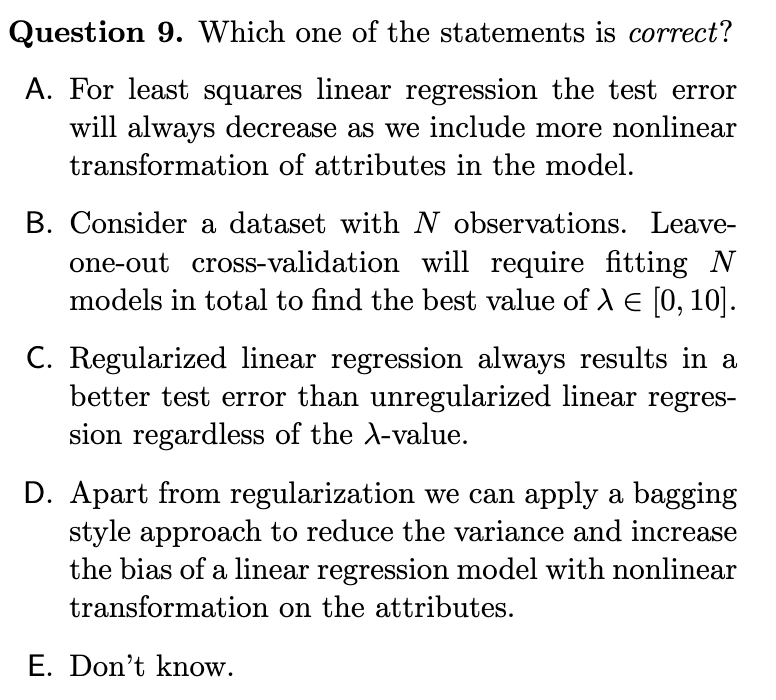
\includegraphics[width=0.65\linewidth]{images/Type A.png}
    \caption{Unpaired text example}
    \label{fig:typeA}
\end{figure}

\begin{figure}[h]
    \centering
    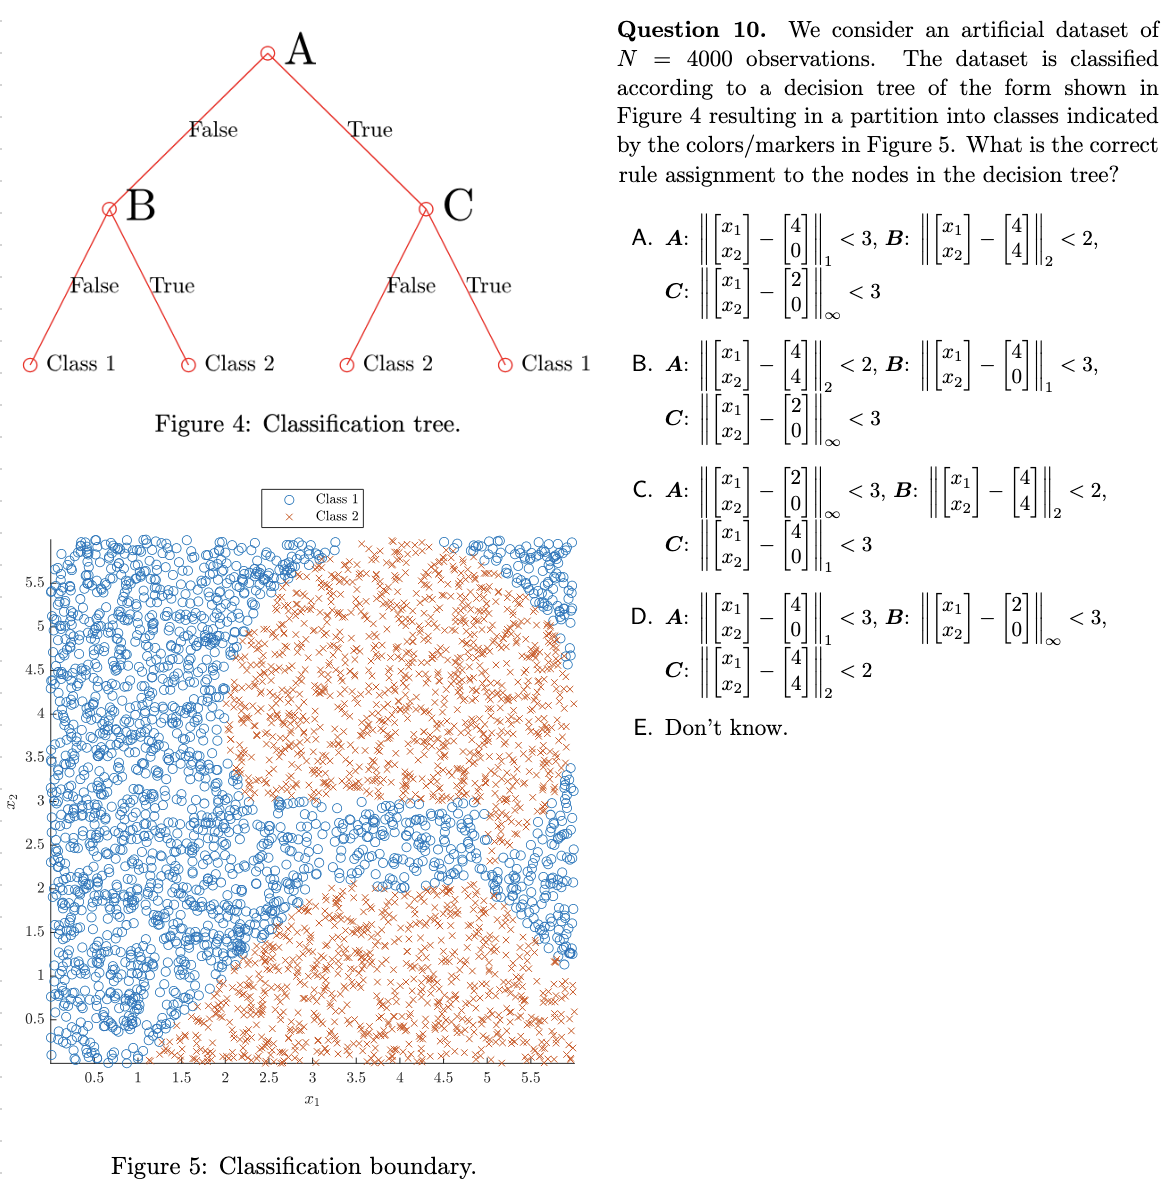
\includegraphics[width=0.75\linewidth]{images/Type B.png}
    \caption{Unpaired image example}
    \label{fig:typeB}
\end{figure}

\begin{figure}[h]
    \centering
    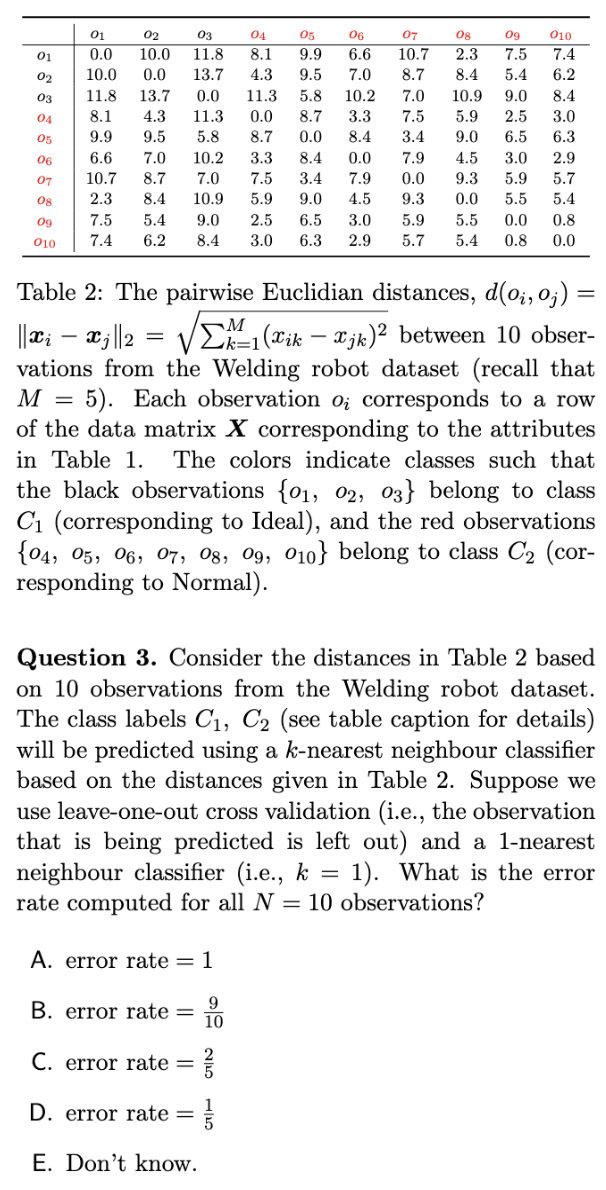
\includegraphics[width=0.60\linewidth]{images/Type C.png}
    \caption{Paired question example}
    \label{fig:typeC}
\end{figure}

\end{document}